\chapter{Entwicklung der Klassifikatoren}

\section{Merkmalsextraktion}
Bla bla bla

\section{Mindesabstand Klassifikator}

\subsection{Euklidischer Abstand}

\begin{table}[ht]
\centering
\begin{tabular}{| l | r |}
    \hline
    Accuracy                & 84.44\% \\
    Recall                  & 100.00\% \\
    Cars prediction value   & 76.27\% \\
    Trucks prediction value & 100.00\% \\
    F1                      & 86.54\% \\
    \hline
\end{tabular}
\caption{Bewertungsmetriken des Mindestabstand Klassifikators (Euklidischer
Abstand)}
\label{tab:euklid}
\end{table}

\begin{figure}[ht]
\centering
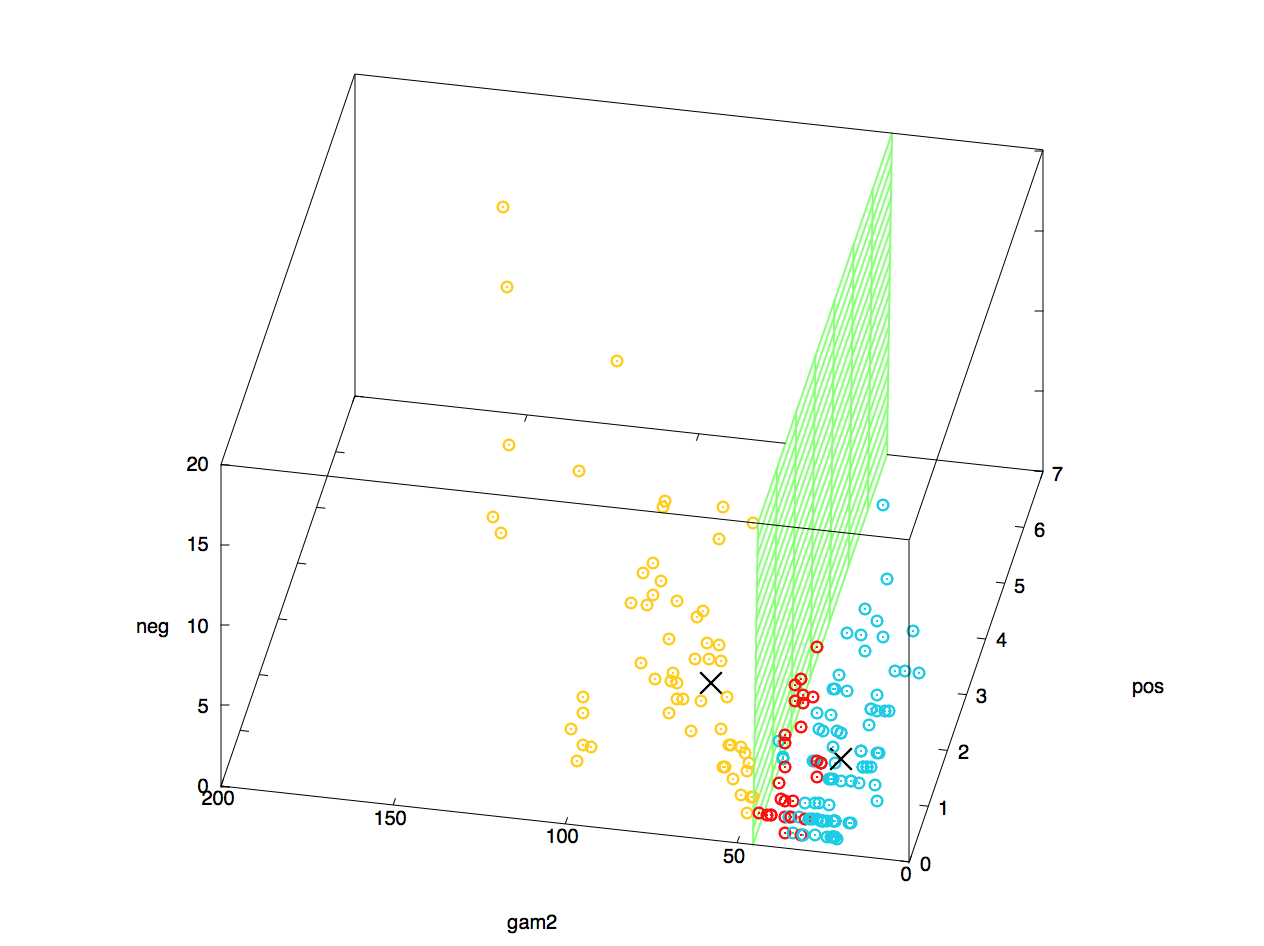
\includegraphics[width=1\textwidth]{mindestabstandEuklid}
\caption{Ergebnis der Pr\"ufung des Mindestabstand Klassifikators (Euklidischer
Abstand)}
\label{fig:euklid}
\end{figure}

\subsection{Mahalanobis-Distanz}

\begin{table}[ht]
\centering
\begin{tabular}{| l | r |}
    \hline
    Accuracy                & 86.11\% \\
    Recall                  & 95.56\% \\
    Cars prediction value   & 80.37\% \\
    Trucks prediction value & 94.52\% \\
    F1                      & 87.31\% \\
    \hline
\end{tabular}
\caption{Bewertungsmetriken des Mindestabstand Klassifikators (Mahalanobis-%
Distanz)}
\label{tab:mahalanobis}
\end{table}

\begin{figure}[ht]
\centering
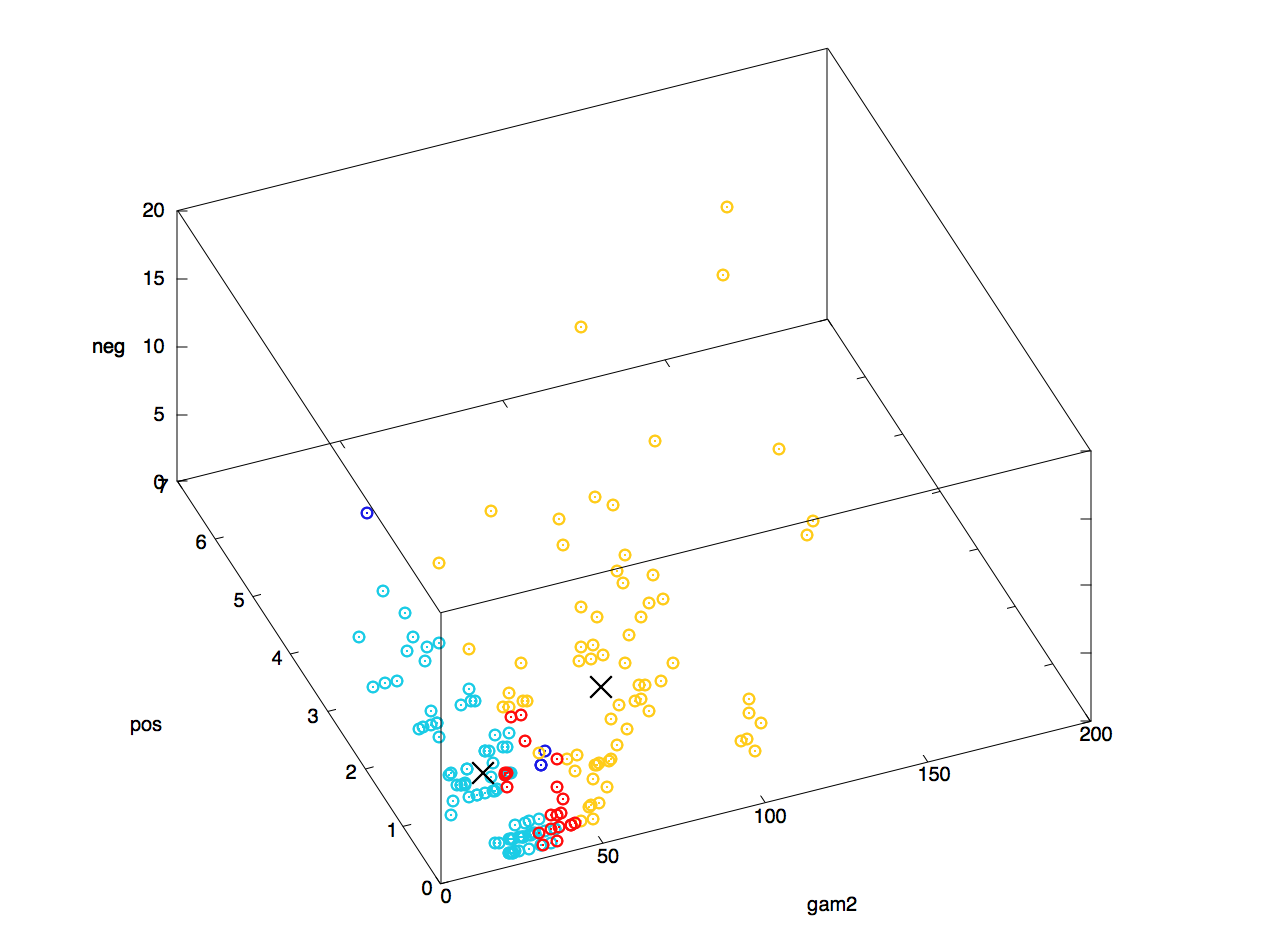
\includegraphics[width=1\textwidth]{mindestabstandMahalanobis}
\caption{Ergebnis der Pr\"ufung des Mindestabstand Klassifikators (Mahalanobis-%
Distanz)}
\label{fig:mahalanobis}
\end{figure}

\section{Naiver Bayes-Klassifikator}

\begin{table}[ht]
\centering
\begin{tabular}{| l | r |}
    \hline
    Accuracy                & 97.22\% \\
    Recall                  & 96.67\% \\
    Cars prediction value   & 97.75\% \\
    Trucks prediction value & 96.70\% \\
    F1                      & 97.21\% \\
    \hline
\end{tabular}
\caption{Bewertungsmetriken des naiven Bayes-Klassifikators}
\label{tab:bayes}
\end{table}

\begin{figure}[ht]
\centering
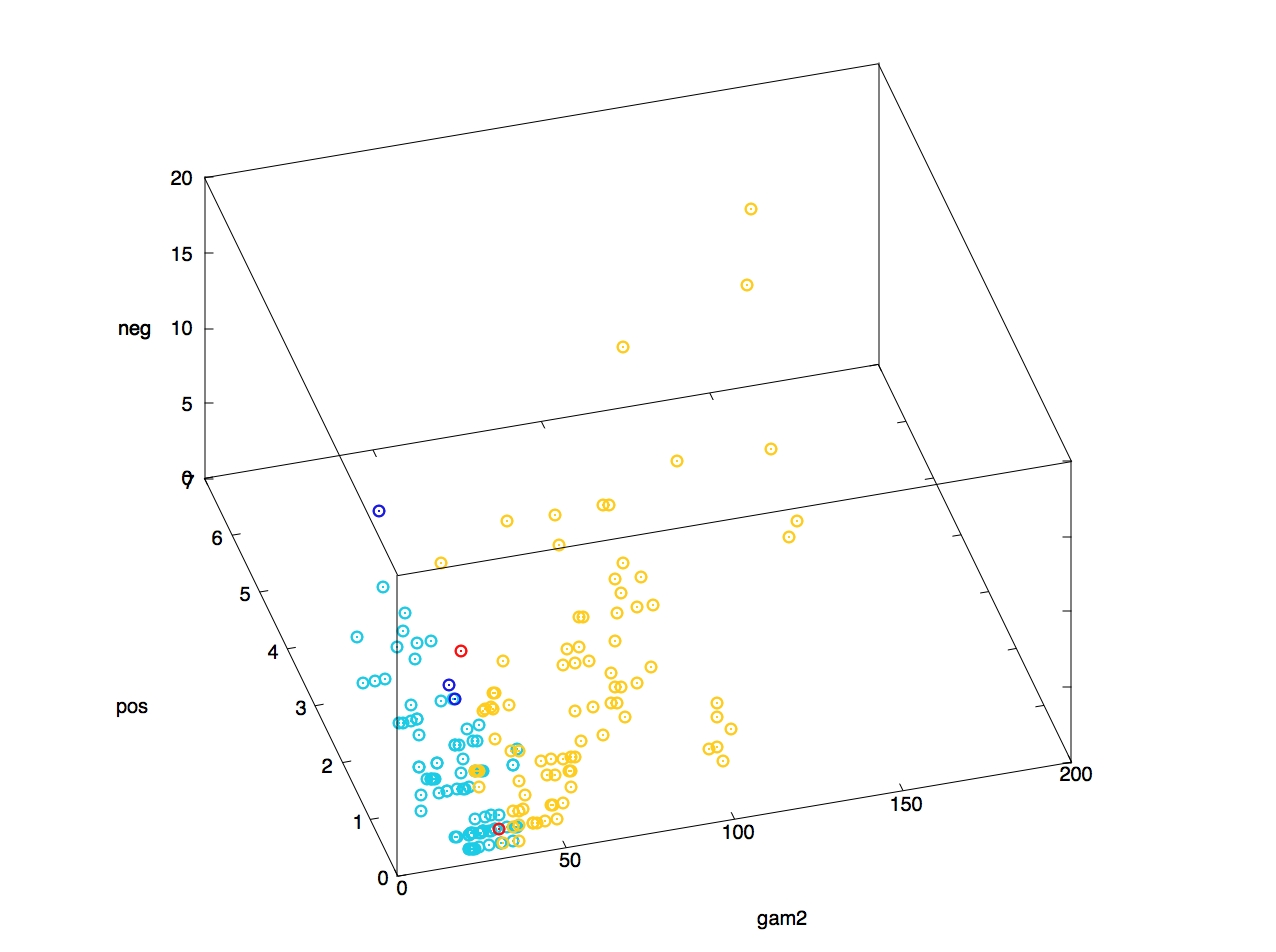
\includegraphics[width=1\textwidth]{naiverBayes}
\caption{Ergebnis der Pr\"ufung des naiven Bayes-Klassifikators}
\label{fig:bayes}
\end{figure}

\section{Neuronales Netz}

\begin{table}[ht]
\centering
\begin{tabular}{| l | r |}
    \hline
    Accuracy                & 93.33\% \\
    Recall                  & 93.33\% \\
    Cars prediction value   & 93.33\% \\
    Trucks prediction value & 93.33\% \\
    F1                      & 93.33\% \\
    \hline
\end{tabular}
\caption{Bewertungsmetriken des neuronalen Netzes}
\label{tab:netz}
\end{table}

\begin{figure}[ht]
\centering
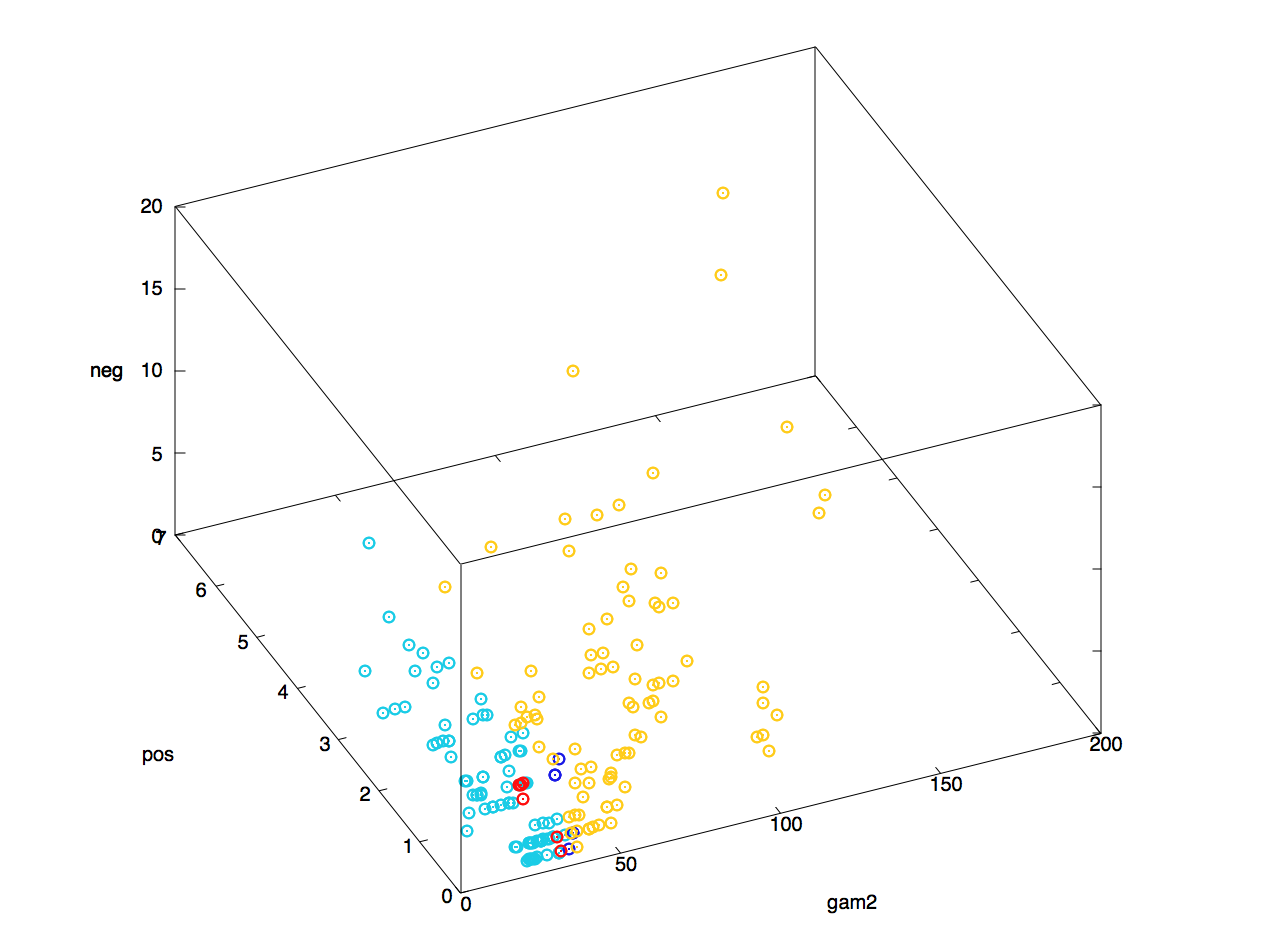
\includegraphics[width=1\textwidth]{neuronalesNetz}
\caption{Ergebnis der Pr\"ufung des neuronalen Netzes}
\label{fig:netz}
\end{figure}